\chapter{浮動小数点数と固定小数点数についての基礎知識}
\label{chap:基礎知識1}
計算機内部で扱う数値には二つの表現方法がある.
それぞれの表現方法を固定小数点数がと浮動小数点数という.これらの表現方法について説明する.
固定小数点数,浮動小数点数はともに数を計算機が記憶しておくための数の表現方法である.

\section{固定小数点}
固定小数点数は,与えられたbit数に対して,そのうち小数部にいくつのbitを割り当てるのかを決めて残りのbitを整数部に割り当てて数を表現する方法である.
例として,$N \in \N$として計算機の中で$N$bitが数字を記憶するために与えられているとする.
そのうち,$m \ (m < N)$bitを小数部に割り当てた固定小数点数$a$は,符号を考えない場合以下のように表すことができる:

\begin{align}
    a = a_{N-m-1} 2^{N-m-1} + a_{N-m-2} 2^{N-m-2} + \cdots + a_1 2^1 + a_0 2^0 + a_{-1} 2^{-1} + \cdots + a_{-m} 2^{-m}.
\end{align}
ただし,$a_{i} \ (i = N-m-1,N-m-2,\dots,1,0,-1,\dots,-m)$は$0$または$1$の値を取る.
\begin{figure}[H]
    \centering
    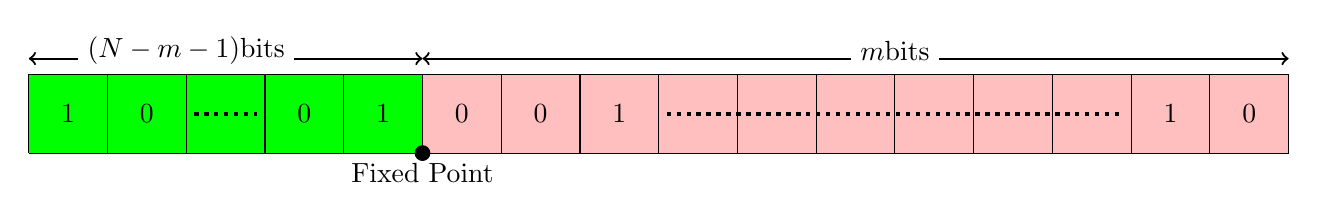
\begin{tikzpicture}
        \fill[green] (0,0) rectangle (5,1);
        \fill[pink] (5,0) rectangle (16,1);
        \draw (0,0) grid (16,1);
        \fill (5,0) circle [radius=0.1] node [below] {Fixed Point};
        \draw[ultra thick, dotted] (2.1,0.5) -- (2.9,0.5);
        \node [anchor=center] at (0.5,0.5) {1};
        \node [anchor=center] at (1.5,0.5) {0};
        \node [anchor=center] at (3.5,0.5) {0};
        \node [anchor=center] at (4.5,0.5) {1};
        \node [anchor=center] at (5.5,0.5) {0};
        \node [anchor=center] at (6.5,0.5) {0};
        \node [anchor=center] at (7.5,0.5) {1};
        \draw[ultra thick, dotted] (8.1,0.5) -- (13.9,0.5);
        \node [anchor=center] at (14.5,0.5) {1};
        \node [anchor=center] at (15.5,0.5) {0};
        \draw[<->,thick] (0,1.2) -- (5,1.2);
        \draw (2,1.3) node[fill=white] {$(N-m-1)$bits};
        \draw[<->,thick] (5,1.2) -- (16,1.2);
        \draw (11,1.3) node[fill=white] {$m$bits};
    \end{tikzpicture}
    \caption{$N$bitの符号なし固定小数点のイメージ図}
    \label{fig:fixedpointnumber_unsigned}
\end{figure}
また,符号付き固定小数点の場合,符号に$1$bit割り当てるため整数部が$N-m-2$bitとなる.
\begin{figure}[H]
    \centering
    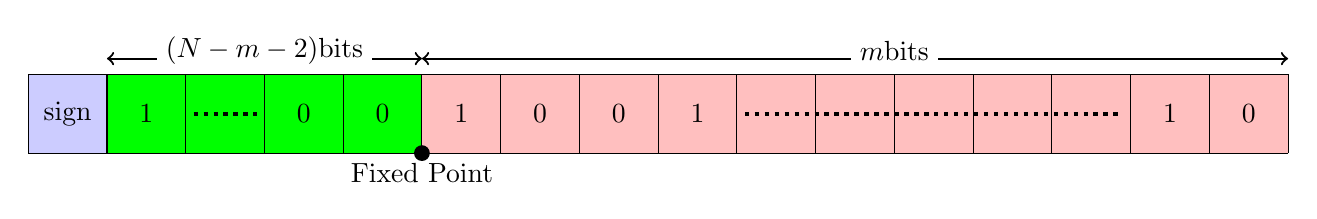
\begin{tikzpicture}
        \fill[green] (1,0) rectangle (5,1);
        \fill[pink] (5,0) rectangle (16,1);
        \fill[blue, opacity=0.2] (0,0) rectangle (1,1);
        \draw (0,0) grid (16,1);
        \fill (5,0) circle [radius=0.1] node [below] {Fixed Point};
        \draw[ultra thick, dotted] (2.1,0.5) -- (2.9,0.5);
        \node [anchor=center] at (0.5,0.5) {sign};
        \node [anchor=center] at (1.5,0.5) {1};
        \node [anchor=center] at (3.5,0.5) {0};
        \node [anchor=center] at (4.5,0.5) {0};
        \node [anchor=center] at (5.5,0.5) {1};
        \node [anchor=center] at (6.5,0.5) {0};
        \node [anchor=center] at (7.5,0.5) {0};
        \node [anchor=center] at (8.5,0.5) {1};
        \draw[ultra thick, dotted] (9.1,0.5) -- (13.9,0.5);
        \node [anchor=center] at (14.5,0.5) {1};
        \node [anchor=center] at (15.5,0.5) {0};
        \draw[<->,thick] (1,1.2) -- (5,1.2);
        \draw[<->,thick] (5,1.2) -- (16,1.2);
        \draw (3,1.3) node[fill=white] {$(N-m-2)$bits};
        \draw (11,1.3) node[fill=white] {$m$bits};
    \end{tikzpicture}
    \caption{$N$bitの符号付き固定小数点のイメージ図}
    \label{fig:fixedpointnumber_signed}
\end{figure}
本論文では,$N$bitの符号付き固定小数点で小数部に$m$bit,整数部に$(N-m-2)$bitを割り当てた固定小数点を,
\begin{equation}
    \text{Q}(N-m-2)\text{f}m
\end{equation}
と表す.
例えば,Q11f52は符号に1bit,小数部に52bit,整数部に11bitを割り当てた固定小数点数のことを表す.
\section{浮動小数点}
浮動小数点は,与えられたbit数に対して,bitを仮数部と指数部にわけて数を表現する方法である.
仮数部の数を$m$,指数部の数を$e$とすると浮動小数点$b$は,以下の様に表現することができる:
\begin{align}
    b = m \times 2^e.
\end{align}
ここで$m,e$はともに2進数の数である.
浮動小数点については,国際的な規格があり,割り当てられるbit数が32bit,64bitのものをそれぞれ単精度浮動小数点(Float32),倍精度浮動小数点(Float64)という.
それぞれの浮動小数点数の仮数部と指数部のbit数は以下の表のように決められている:
\begin{table}[H]
    \centering
    \caption{単精度浮動小数点(Float32)と倍精度浮動小数点(Float64)の仮数部と指数部のbit数}
    \begin{tabular}{c|c|c}   
     & 仮数部 & 指数部 \\ \hline
    Float32 & 23bit & 8bit \\ 
    Float64 & 52bit & 11bit
    \end{tabular}
    \label{tab:Float32_Float64_bit}
\end{table}
浮動小数点はbit数によって表現出来る数の範囲が異なる.
単精度浮動小数点と倍精度浮動小数点では以下の様になる:
\begin{table}[H]
    \centering
    \caption{単精度浮動小数点と倍精度浮動小数点の表現可能な数の範囲}
    \begin{tabular}{c|c|c|c}   
     & 最大値 & 最小値 & 0に最も近い数 \\ \hline
    Float32 & & & \\
    Float64 & & &
    \end{tabular}
    \label{tab:Float32_Float64_range}
\end{table}